To validate the feasibility of both mPAI for quantifying the expression of multiple immune checkpoint receptors and PAI with soluble PD1 to measure receptor availability, we first conducted diffusion experiments
in tissue mimicking phantoms without cells. These experiments were designed to determine the diffusion
coefficients and corresponding diffusion times of fluorescently labeled imaging agents. The results 
informed the appropriate incubation times needed before imaging experiments in tissue mimicking 
phantoms with tumor cells.

In biological systems, molecular diffusion arises from the random thermal motion of particles and
is a fundamental mechanism that governs the transport of substances within tissues. This process is
particularly critical in the context of molecular imaging, where the spatial and temporal distribution
of imaging agents determines the accuracy of quantitative assessments.

To characterize diffusion behavior \textit{in vitro}, we used the cell-free, agarose-based 
tissue mimicking phantoms whose protocol is outlined in Section~\ref{sec:chapter2_methods}. Fluorescent images were acquired using the Pearl imaging system, and the images were analyzed using MATLAB.
A region of interest (ROI) was defined around the central hole where the fluorescent agent was
introduced, using an ROI generator implemented in MATLAB. To account for variability in the shape
of the holes in the agar, the ROI was rotated at four angles: $0^\circ, 45^\circ, 90^\circ,$ 
and $135^\circ$. Pixel intensities within the ROI were summed column-wise to generate
one-dimensional intensity profiles for each orientation.

To quantify radial diffusion from the hole containing the dye at the center of the well, the full-width at half-maximum (FWHM) method was applied after subtracting the background signal acquired before dye addition. The diffusion distance at time, $t$, was therefore determined based on the width of the profile at half its maximum intensity, 
as illustrated in Figure ~\ref{fig:full_width_half_maximum}. 


\begin{wrapfigure}{R}{0.7\textwidth}
    \vspace{-1em} % space above
    \hspace{2em}  % left buffer
    \begin{minipage}{0.6\textwidth} % slightly smaller than 0.62
        \centering
        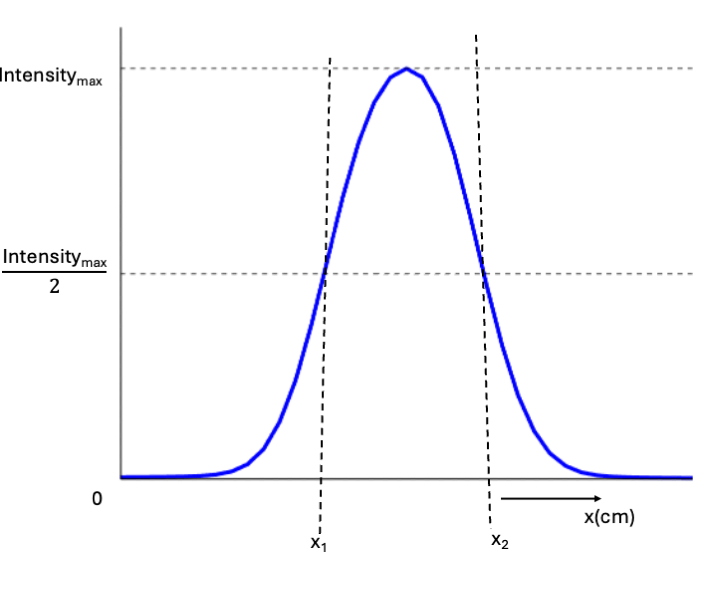
\includegraphics[width=\linewidth]{figures/fwhm_plots.png}
        \captionsetup{justification=raggedright, singlelinecheck=false}
        \caption[FWHM technique]{\textbf{FWHM technique illustration.} The curve shows fluorescence intensity as a function of $x$ (cm). FWHM is the width at half-maximum between $x_1$ and $x_2$.}
        \label{fig:full_width_half_maximum}
        \vspace{1em} % bottom buffer
    \end{minipage}
\end{wrapfigure}




To determine the diffusion coefficient, we modeled the spread of dye within the agarose phantom as a
two-dimensional random walk originating from the hole that contains the dye. The diffusion behavior was quantified using the mean squared displacement (MSD) relation shown in Equation~\ref{eq:msd}:

\begin{equation}
\label{eq:msd}
    \langle r^2 \rangle = 4Dt
\end{equation}
where $D$ is the diffusion coefficient $\left( \mathrm{cm}^2/\mathrm{s} \right)$ and $t$ is the time of image 
acquisition(s).

The experimental time ($t_{exp}$) required for the fluorescent antibody to distribute evenly throughout the 
tissue mimicking phantom was determined using Equation~\ref{eq:msd}, but using the depth of the tissue mimicking 
phantom ($x = 0.106 cm$) and the experimentally determined diffusion coefficient ($D$) above:
\begin{equation}
\label{eq:texp}
    t_{exp} = \frac{x^2}{4D} = \frac{\left(0.106cm\right)^2}{4D}
\end{equation}

Figure ~\ref{fig:representative_of_difusion_time} presents representative ROI images rotated at four angles ($0^\circ, 45^\circ, 90^\circ,$ and $135^\circ$), together with the corresponding intensity peak profiles and $\langle r^2 \rangle$ versus $time$ plots used to calculate the diffusion coefficients.

\begin{figure}[H]
    \centering
    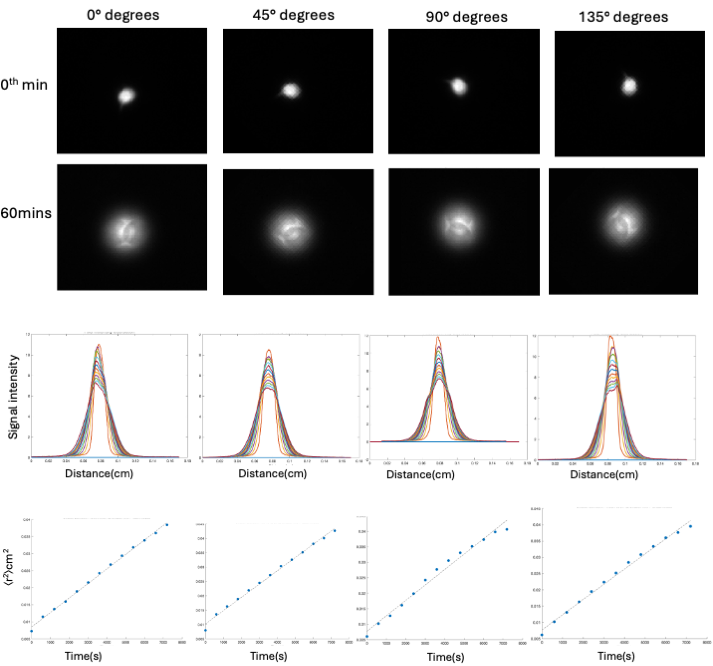
\includegraphics[width=0.98\linewidth]{figures/representative_of difusion_time.png}
    \captionsetup{justification=raggedright,singlelinecheck=false}
    \caption[Representative diffusion analysis]{\textbf{Representative diffusion analysis across four angular directions ($0^\circ, 45^\circ, 90^\circ$, and $135^\circ$)}. 
    Top panels show fluorescence images of the ROI at $0$ and $60$ minutes. Middle panels display signal 
    intensity profiles as a function of distance from the center, extracted from each time point and angle. 
    Bottom panels present mean squared displacement, $\langle r^2 \rangle$, versus time plots corresponding to each orientation, 
    used to calculate diffusion coefficients.}
    \label{fig:representative_of_difusion_time}
\end{figure}


For the mPAI experiments, three monoclonal antibodies were used as targeted imaging agents: anti-PD1 was conjugated to IR680, anti-PDL1 to AF750, and anti-CD80 to AF700. An untargeted antibody (IgG) was labeled with IR800. For the PAI experiment involving soluble proteins, a soluble PD1 protein was labeled with IR800 and paired with free IR680 as an untargeted control. These fluorophore-protein pairings were selected based on preliminary liquid phantom experiments (described in Chapter ~\ref{ch:chapter3}) that evaluated fluorescence intensity, linearity, and spectral interference across the detection channels of the Pearl imaging system.